\documentclass[twoside]{book}

% Packages required by doxygen
\usepackage{fixltx2e}
\usepackage{calc}
\usepackage{doxygen}
\usepackage[export]{adjustbox} % also loads graphicx
\usepackage{graphicx}
\usepackage[utf8]{inputenc}
\usepackage{makeidx}
\usepackage{multicol}
\usepackage{multirow}
\PassOptionsToPackage{warn}{textcomp}
\usepackage{textcomp}
\usepackage[nointegrals]{wasysym}
\usepackage[table]{xcolor}

% Font selection
\usepackage[T1]{fontenc}
\usepackage[scaled=.90]{helvet}
\usepackage{courier}
\usepackage{amssymb}
\usepackage{sectsty}
\renewcommand{\familydefault}{\sfdefault}
\allsectionsfont{%
  \fontseries{bc}\selectfont%
  \color{darkgray}%
}
\renewcommand{\DoxyLabelFont}{%
  \fontseries{bc}\selectfont%
  \color{darkgray}%
}
\newcommand{\+}{\discretionary{\mbox{\scriptsize$\hookleftarrow$}}{}{}}

% Page & text layout
\usepackage{geometry}
\geometry{%
  a4paper,%
  top=2.5cm,%
  bottom=2.5cm,%
  left=2.5cm,%
  right=2.5cm%
}
\tolerance=750
\hfuzz=15pt
\hbadness=750
\setlength{\emergencystretch}{15pt}
\setlength{\parindent}{0cm}
\setlength{\parskip}{3ex plus 2ex minus 2ex}
\makeatletter
\renewcommand{\paragraph}{%
  \@startsection{paragraph}{4}{0ex}{-1.0ex}{1.0ex}{%
    \normalfont\normalsize\bfseries\SS@parafont%
  }%
}
\renewcommand{\subparagraph}{%
  \@startsection{subparagraph}{5}{0ex}{-1.0ex}{1.0ex}{%
    \normalfont\normalsize\bfseries\SS@subparafont%
  }%
}
\makeatother

% Headers & footers
\usepackage{fancyhdr}
\pagestyle{fancyplain}
\fancyhead[LE]{\fancyplain{}{\bfseries\thepage}}
\fancyhead[CE]{\fancyplain{}{}}
\fancyhead[RE]{\fancyplain{}{\bfseries\leftmark}}
\fancyhead[LO]{\fancyplain{}{\bfseries\rightmark}}
\fancyhead[CO]{\fancyplain{}{}}
\fancyhead[RO]{\fancyplain{}{\bfseries\thepage}}
\fancyfoot[LE]{\fancyplain{}{}}
\fancyfoot[CE]{\fancyplain{}{}}
\fancyfoot[RE]{\fancyplain{}{\bfseries\scriptsize Generated by Doxygen }}
\fancyfoot[LO]{\fancyplain{}{\bfseries\scriptsize Generated by Doxygen }}
\fancyfoot[CO]{\fancyplain{}{}}
\fancyfoot[RO]{\fancyplain{}{}}
\renewcommand{\footrulewidth}{0.4pt}
\renewcommand{\chaptermark}[1]{%
  \markboth{#1}{}%
}
\renewcommand{\sectionmark}[1]{%
  \markright{\thesection\ #1}%
}

% Indices & bibliography
\usepackage{natbib}
\usepackage[titles]{tocloft}
\setcounter{tocdepth}{3}
\setcounter{secnumdepth}{5}
\makeindex

% Hyperlinks (required, but should be loaded last)
\usepackage{ifpdf}
\ifpdf
  \usepackage[pdftex,pagebackref=true]{hyperref}
\else
  \usepackage[ps2pdf,pagebackref=true]{hyperref}
\fi
\hypersetup{%
  colorlinks=true,%
  linkcolor=blue,%
  citecolor=blue,%
  unicode%
}

% Custom commands
\newcommand{\clearemptydoublepage}{%
  \newpage{\pagestyle{empty}\cleardoublepage}%
}

\usepackage{caption}
\captionsetup{labelsep=space,justification=centering,font={bf},singlelinecheck=off,skip=4pt,position=top}

%===== C O N T E N T S =====

\begin{document}

% Titlepage & ToC
\hypersetup{pageanchor=false,
             bookmarksnumbered=true,
             pdfencoding=unicode
            }
\pagenumbering{alph}
\begin{titlepage}
\vspace*{7cm}
\begin{center}%
{\Large U\+Model }\\
\vspace*{1cm}
{\large Generated by Doxygen 1.8.14}\\
\end{center}
\end{titlepage}
\clearemptydoublepage
\pagenumbering{roman}
\tableofcontents
\clearemptydoublepage
\pagenumbering{arabic}
\hypersetup{pageanchor=true}

%--- Begin generated contents ---
\chapter{Hierarchical Index}
\section{Class Hierarchy}
This inheritance list is sorted roughly, but not completely, alphabetically\+:\begin{DoxyCompactList}
\item \contentsline{section}{U\+Model\+:\+:\+\_\+\+O\+D\+E\+P\+AR}{\pageref{structUModel_1_1__ODEPAR}}{}
\item \contentsline{section}{U\+Model\+:\+:\+\_\+\+R\+E\+AC}{\pageref{structUModel_1_1__REAC}}{}
\item \contentsline{section}{U\+Model\+:\+:\+\_\+\+S\+P\+ES}{\pageref{structUModel_1_1__SPES}}{}
\item \contentsline{section}{U\+Model\+:\+:\+\_\+\+T\+CV}{\pageref{structUModel_1_1__TCV}}{}
\item ctype\begin{DoxyCompactList}
\item \contentsline{section}{Filter\+Character}{\pageref{classFilterCharacter}}{}
\end{DoxyCompactList}
\item exception\begin{DoxyCompactList}
\item \contentsline{section}{U\+Exception}{\pageref{classUException}}{}
\end{DoxyCompactList}
\item \contentsline{section}{U\+Model}{\pageref{classUModel}}{}
\end{DoxyCompactList}

\chapter{Class Index}
\section{Class List}
Here are the classes, structs, unions and interfaces with brief descriptions\+:\begin{DoxyCompactList}
\item\contentsline{section}{\hyperlink{structUModel_1_1__ODEPAR}{U\+Model\+::\+\_\+\+O\+D\+E\+P\+AR} \\*Parameter for O\+DE Solver }{\pageref{structUModel_1_1__ODEPAR}}{}
\item\contentsline{section}{\hyperlink{structUModel_1_1__REAC}{U\+Model\+::\+\_\+\+R\+E\+AC} }{\pageref{structUModel_1_1__REAC}}{}
\item\contentsline{section}{\hyperlink{structUModel_1_1__SPES}{U\+Model\+::\+\_\+\+S\+P\+ES} }{\pageref{structUModel_1_1__SPES}}{}
\item\contentsline{section}{\hyperlink{structUModel_1_1__TCV}{U\+Model\+::\+\_\+\+T\+CV} }{\pageref{structUModel_1_1__TCV}}{}
\item\contentsline{section}{\hyperlink{classFilterCharacter}{Filter\+Character} }{\pageref{classFilterCharacter}}{}
\item\contentsline{section}{\hyperlink{classUException}{U\+Exception} \\*\hyperlink{classUException}{U\+Exception} class exception may be throwed by \hyperlink{classUModel}{U\+Model} class method }{\pageref{classUException}}{}
\item\contentsline{section}{\hyperlink{classUModel}{U\+Model} \\*\hyperlink{classUModel}{U\+Model} Class }{\pageref{classUModel}}{}
\end{DoxyCompactList}

\chapter{Class Documentation}
\hypertarget{structUModel_1_1__ODEPAR}{}\section{U\+Model\+:\+:\+\_\+\+O\+D\+E\+P\+AR Struct Reference}
\label{structUModel_1_1__ODEPAR}\index{U\+Model\+::\+\_\+\+O\+D\+E\+P\+AR@{U\+Model\+::\+\_\+\+O\+D\+E\+P\+AR}}


parameter for O\+DE Solver  




{\ttfamily \#include $<$U\+Model.\+h$>$}

\subsection*{Public Attributes}
\begin{DoxyCompactItemize}
\item 
\mbox{\Hypertarget{structUModel_1_1__ODEPAR_a5fc201c270bf6a304386f82134417440}\label{structUModel_1_1__ODEPAR_a5fc201c270bf6a304386f82134417440}} 
void($\ast$ {\bfseries D\+IF} )(int $\ast$N, double $\ast$\hyperlink{structUModel_1_1__ODEPAR_a407dfd8303377097296a7288d964555e}{T}, double $\ast$Y, double $\ast$Y\+D\+OT, double $\ast$R\+P\+AR, int $\ast$I\+P\+AR) =N\+U\+LL
\item 
\mbox{\Hypertarget{structUModel_1_1__ODEPAR_a3485fd61d0d7a719aaa1356d96e7ea11}\label{structUModel_1_1__ODEPAR_a3485fd61d0d7a719aaa1356d96e7ea11}} 
double $\ast$ {\bfseries Y}
\item 
\mbox{\Hypertarget{structUModel_1_1__ODEPAR_a407dfd8303377097296a7288d964555e}\label{structUModel_1_1__ODEPAR_a407dfd8303377097296a7288d964555e}} 
double \hyperlink{structUModel_1_1__ODEPAR_a407dfd8303377097296a7288d964555e}{T}
\begin{DoxyCompactList}\small\item\em init time \end{DoxyCompactList}\item 
\mbox{\Hypertarget{structUModel_1_1__ODEPAR_af1fbeec8d118f47f0aaa246e462892e4}\label{structUModel_1_1__ODEPAR_af1fbeec8d118f47f0aaa246e462892e4}} 
double \hyperlink{structUModel_1_1__ODEPAR_af1fbeec8d118f47f0aaa246e462892e4}{T\+O\+UT}
\begin{DoxyCompactList}\small\item\em end time \end{DoxyCompactList}\item 
\mbox{\Hypertarget{structUModel_1_1__ODEPAR_a43abf4534531cc6dad4b3ad5693b8a37}\label{structUModel_1_1__ODEPAR_a43abf4534531cc6dad4b3ad5693b8a37}} 
int {\bfseries N\+EQ}
\item 
\mbox{\Hypertarget{structUModel_1_1__ODEPAR_a4d3aca7b7e2f6a5fc5c7c5d46ad5cc94}\label{structUModel_1_1__ODEPAR_a4d3aca7b7e2f6a5fc5c7c5d46ad5cc94}} 
int $\ast$ {\bfseries I\+W\+O\+RK}
\item 
\mbox{\Hypertarget{structUModel_1_1__ODEPAR_ae61dee0c304fe6e1ff23d384e2f6f22e}\label{structUModel_1_1__ODEPAR_ae61dee0c304fe6e1ff23d384e2f6f22e}} 
int {\bfseries L\+IW}
\item 
\mbox{\Hypertarget{structUModel_1_1__ODEPAR_afc3d67c6cd232cd64f5af637b8dac59a}\label{structUModel_1_1__ODEPAR_afc3d67c6cd232cd64f5af637b8dac59a}} 
double $\ast$ {\bfseries R\+W\+O\+RK}
\item 
\mbox{\Hypertarget{structUModel_1_1__ODEPAR_a5fc87aa51fed5065bb2ecb25d9df13d1}\label{structUModel_1_1__ODEPAR_a5fc87aa51fed5065bb2ecb25d9df13d1}} 
int {\bfseries L\+RW}
\item 
\mbox{\Hypertarget{structUModel_1_1__ODEPAR_a726749046d89df737da64ab06b3498b5}\label{structUModel_1_1__ODEPAR_a726749046d89df737da64ab06b3498b5}} 
int {\bfseries I\+T\+OL} =1
\item 
\mbox{\Hypertarget{structUModel_1_1__ODEPAR_ab86524dfb4b14f806411bf3a7028f658}\label{structUModel_1_1__ODEPAR_ab86524dfb4b14f806411bf3a7028f658}} 
double {\bfseries R\+T\+OL} = 1.\+0\+E-\/5
\item 
\mbox{\Hypertarget{structUModel_1_1__ODEPAR_a9267fbaa8a77c5604000a9ae11a30d04}\label{structUModel_1_1__ODEPAR_a9267fbaa8a77c5604000a9ae11a30d04}} 
double {\bfseries A\+T\+OL} = 1.\+0\+E-\/20
\item 
\mbox{\Hypertarget{structUModel_1_1__ODEPAR_a1a6d5be08279269961e73732a39c5989}\label{structUModel_1_1__ODEPAR_a1a6d5be08279269961e73732a39c5989}} 
int {\bfseries I\+T\+A\+SK} = 1
\item 
\mbox{\Hypertarget{structUModel_1_1__ODEPAR_abc1065ef47e6f953d5ea1cccb29e0126}\label{structUModel_1_1__ODEPAR_abc1065ef47e6f953d5ea1cccb29e0126}} 
int {\bfseries I\+S\+T\+A\+TE} = 1
\item 
\mbox{\Hypertarget{structUModel_1_1__ODEPAR_aab15af2cf0efcc50857822da6f84ca66}\label{structUModel_1_1__ODEPAR_aab15af2cf0efcc50857822da6f84ca66}} 
int {\bfseries I\+O\+PT} =1
\item 
\mbox{\Hypertarget{structUModel_1_1__ODEPAR_accabc313291f45ab645ac25651e262b4}\label{structUModel_1_1__ODEPAR_accabc313291f45ab645ac25651e262b4}} 
void($\ast$ {\bfseries J\+AC} )(int $\ast$N, double $\ast$\hyperlink{structUModel_1_1__ODEPAR_a407dfd8303377097296a7288d964555e}{T}, double $\ast$Y, int $\ast$ML, int $\ast$MU, double $\ast$PD, int $\ast$N\+R\+W\+O\+R\+K\+PD, double $\ast$R\+P\+AR, int $\ast$I\+P\+AR) =N\+U\+LL
\item 
\mbox{\Hypertarget{structUModel_1_1__ODEPAR_a2ea8e03f8db5564e1eadb921ee70f8ff}\label{structUModel_1_1__ODEPAR_a2ea8e03f8db5564e1eadb921ee70f8ff}} 
int {\bfseries MF} = 22
\item 
\mbox{\Hypertarget{structUModel_1_1__ODEPAR_aa840a6bd72e41aeb6d8300e68404216a}\label{structUModel_1_1__ODEPAR_aa840a6bd72e41aeb6d8300e68404216a}} 
int $\ast$ {\bfseries I\+P\+AR} = N\+U\+LL
\item 
\mbox{\Hypertarget{structUModel_1_1__ODEPAR_a60121e6d6cfd33fa2acabd7d5cb2aa17}\label{structUModel_1_1__ODEPAR_a60121e6d6cfd33fa2acabd7d5cb2aa17}} 
double $\ast$ {\bfseries R\+P\+AR} = N\+U\+LL
\end{DoxyCompactItemize}


\subsection{Detailed Description}
parameter for O\+DE Solver 

see more in any introduction about O\+DE Solver. \begin{DoxyNote}{Note}
I\+P\+AR and R\+P\+AR are array send to O\+DE Solver and Callback Function, and they can be used to record for example address of data which stored additional information required. 
\end{DoxyNote}


Definition at line 114 of file U\+Model.\+h.



The documentation for this struct was generated from the following file\+:\begin{DoxyCompactItemize}
\item 
U\+Model.\+h\end{DoxyCompactItemize}

\hypertarget{structUModel_1_1__REAC}{}\section{U\+Model\+:\+:\+\_\+\+R\+E\+AC Struct Reference}
\label{structUModel_1_1__REAC}\index{U\+Model\+::\+\_\+\+R\+E\+AC@{U\+Model\+::\+\_\+\+R\+E\+AC}}


{\ttfamily \#include $<$U\+Model.\+h$>$}

\subsection*{Public Attributes}
\begin{DoxyCompactItemize}
\item 
\mbox{\Hypertarget{structUModel_1_1__REAC_ae92bd72d613da4a5b26ef83b43f6a18e}\label{structUModel_1_1__REAC_ae92bd72d613da4a5b26ef83b43f6a18e}} 
bool \hyperlink{structUModel_1_1__REAC_ae92bd72d613da4a5b26ef83b43f6a18e}{good}
\begin{DoxyCompactList}\small\item\em if false, subpress this reaction \end{DoxyCompactList}\item 
\mbox{\Hypertarget{structUModel_1_1__REAC_ad3c97fb2110c11ae61a93092cbaaccb5}\label{structUModel_1_1__REAC_ad3c97fb2110c11ae61a93092cbaaccb5}} 
int \hyperlink{structUModel_1_1__REAC_ad3c97fb2110c11ae61a93092cbaaccb5}{type}
\begin{DoxyCompactList}\small\item\em reaction type. 1-\/3 for photon/particle ionization. 10 for grain surface reaction. \end{DoxyCompactList}\item 
\mbox{\Hypertarget{structUModel_1_1__REAC_a56e0cd68727bc98da5cb86efb70312ef}\label{structUModel_1_1__REAC_a56e0cd68727bc98da5cb86efb70312ef}} 
int \hyperlink{structUModel_1_1__REAC_a56e0cd68727bc98da5cb86efb70312ef}{R} \mbox{[}6\mbox{]}
\begin{DoxyCompactList}\small\item\em R\mbox{[}0\mbox{]} R\mbox{[}1\mbox{]} record reactants index in S\+P\+ES, R\mbox{[}2\mbox{]}-\/R\mbox{[}5\mbox{]} for resultants. \end{DoxyCompactList}\item 
\mbox{\Hypertarget{structUModel_1_1__REAC_a439bbb6b90bf674559f71fd1b6369018}\label{structUModel_1_1__REAC_a439bbb6b90bf674559f71fd1b6369018}} 
int {\bfseries N\+TR}
\item 
\mbox{\Hypertarget{structUModel_1_1__REAC_a19447fc8849380e2ef254bd99be350b9}\label{structUModel_1_1__REAC_a19447fc8849380e2ef254bd99be350b9}} 
double {\bfseries A\+LF} \mbox{[}5\mbox{]}
\item 
\mbox{\Hypertarget{structUModel_1_1__REAC_a2a7e2012eaee7c7b57b6169d75ed0561}\label{structUModel_1_1__REAC_a2a7e2012eaee7c7b57b6169d75ed0561}} 
double {\bfseries B\+ET} \mbox{[}5\mbox{]}
\item 
\mbox{\Hypertarget{structUModel_1_1__REAC_a2a82372b421f066b7750d8f922efd768}\label{structUModel_1_1__REAC_a2a82372b421f066b7750d8f922efd768}} 
double {\bfseries G\+AM} \mbox{[}5\mbox{]}
\item 
\mbox{\Hypertarget{structUModel_1_1__REAC_ada68e9e548d07943b637c4a3f0884438}\label{structUModel_1_1__REAC_ada68e9e548d07943b637c4a3f0884438}} 
double {\bfseries T\+I\+NT} \mbox{[}5\mbox{]}
\item 
\mbox{\Hypertarget{structUModel_1_1__REAC_ac2993bd9620aeb8dbb01be2865edba28}\label{structUModel_1_1__REAC_ac2993bd9620aeb8dbb01be2865edba28}} 
double {\bfseries T\+E\+ND} \mbox{[}5\mbox{]}
\end{DoxyCompactItemize}


\subsection{Detailed Description}
reactions recoeder 

Definition at line 70 of file U\+Model.\+h.



The documentation for this struct was generated from the following file\+:\begin{DoxyCompactItemize}
\item 
U\+Model.\+h\end{DoxyCompactItemize}

\hypertarget{structUModel_1_1__SPES}{}\section{U\+Model\+:\+:\+\_\+\+S\+P\+ES Struct Reference}
\label{structUModel_1_1__SPES}\index{U\+Model\+::\+\_\+\+S\+P\+ES@{U\+Model\+::\+\_\+\+S\+P\+ES}}
\subsection*{Public Attributes}
\begin{DoxyCompactItemize}
\item 
\mbox{\Hypertarget{structUModel_1_1__SPES_a8ab9e7a46e72a4696be7b5fe061b131d}\label{structUModel_1_1__SPES_a8ab9e7a46e72a4696be7b5fe061b131d}} 
string {\bfseries S\+P\+E\+CI}
\item 
\mbox{\Hypertarget{structUModel_1_1__SPES_ad843966f3d86896a2ed9b5211c6d0e4b}\label{structUModel_1_1__SPES_ad843966f3d86896a2ed9b5211c6d0e4b}} 
double {\bfseries M\+S\+P\+EC}
\item 
\mbox{\Hypertarget{structUModel_1_1__SPES_a02f65715badbc393366111c4dfd062ea}\label{structUModel_1_1__SPES_a02f65715badbc393366111c4dfd062ea}} 
double {\bfseries E\+S\+P\+EC}
\item 
\mbox{\Hypertarget{structUModel_1_1__SPES_a9a249980c66775fd348097ea84cb7faf}\label{structUModel_1_1__SPES_a9a249980c66775fd348097ea84cb7faf}} 
map$<$ string, int $>$ {\bfseries A\+T\+O\+MS}
\item 
\mbox{\Hypertarget{structUModel_1_1__SPES_a4fa48d3c09323f2d7a4057472d9a46d5}\label{structUModel_1_1__SPES_a4fa48d3c09323f2d7a4057472d9a46d5}} 
vector$<$ int $>$ {\bfseries Is}
\item 
\mbox{\Hypertarget{structUModel_1_1__SPES_a7586f67dd5adbd54aa53fdaab24d67ce}\label{structUModel_1_1__SPES_a7586f67dd5adbd54aa53fdaab24d67ce}} 
vector$<$ int $>$ {\bfseries Os}
\end{DoxyCompactItemize}


\subsection{Detailed Description}


Definition at line 54 of file U\+Model.\+h.



The documentation for this struct was generated from the following file\+:\begin{DoxyCompactItemize}
\item 
U\+Model.\+h\end{DoxyCompactItemize}

\hypertarget{structUModel_1_1__TCV}{}\section{U\+Model\+:\+:\+\_\+\+T\+CV Struct Reference}
\label{structUModel_1_1__TCV}\index{U\+Model\+::\+\_\+\+T\+CV@{U\+Model\+::\+\_\+\+T\+CV}}
\subsection*{Public Attributes}
\begin{DoxyCompactItemize}
\item 
\mbox{\Hypertarget{structUModel_1_1__TCV_a339c6e2dedd8ace07b81cf42ec055afc}\label{structUModel_1_1__TCV_a339c6e2dedd8ace07b81cf42ec055afc}} 
double {\bfseries t}
\item 
\mbox{\Hypertarget{structUModel_1_1__TCV_a620c22b9cb5c94cde6735866d869b803}\label{structUModel_1_1__TCV_a620c22b9cb5c94cde6735866d869b803}} 
double {\bfseries NH}
\item 
\mbox{\Hypertarget{structUModel_1_1__TCV_aee45639c774754be614b8c769a13b7d6}\label{structUModel_1_1__TCV_aee45639c774754be614b8c769a13b7d6}} 
double {\bfseries AV}
\item 
\mbox{\Hypertarget{structUModel_1_1__TCV_a22f88d0ab1e7663f245ee75fb87f3fea}\label{structUModel_1_1__TCV_a22f88d0ab1e7663f245ee75fb87f3fea}} 
double {\bfseries Temp}
\item 
\mbox{\Hypertarget{structUModel_1_1__TCV_acebd7387888536f111cc2c70e006e0ba}\label{structUModel_1_1__TCV_acebd7387888536f111cc2c70e006e0ba}} 
double {\bfseries nH}
\item 
\mbox{\Hypertarget{structUModel_1_1__TCV_a1dfc0929143dc175f6a576e340c32f30}\label{structUModel_1_1__TCV_a1dfc0929143dc175f6a576e340c32f30}} 
double $\ast$ {\bfseries K}
\end{DoxyCompactItemize}


\subsection{Detailed Description}


Definition at line 84 of file U\+Model.\+h.



The documentation for this struct was generated from the following file\+:\begin{DoxyCompactItemize}
\item 
U\+Model.\+h\end{DoxyCompactItemize}

\hypertarget{classFilterCharacter}{}\section{Filter\+Character Class Reference}
\label{classFilterCharacter}\index{Filter\+Character@{Filter\+Character}}
Inheritance diagram for Filter\+Character\+:\begin{figure}[H]
\begin{center}
\leavevmode
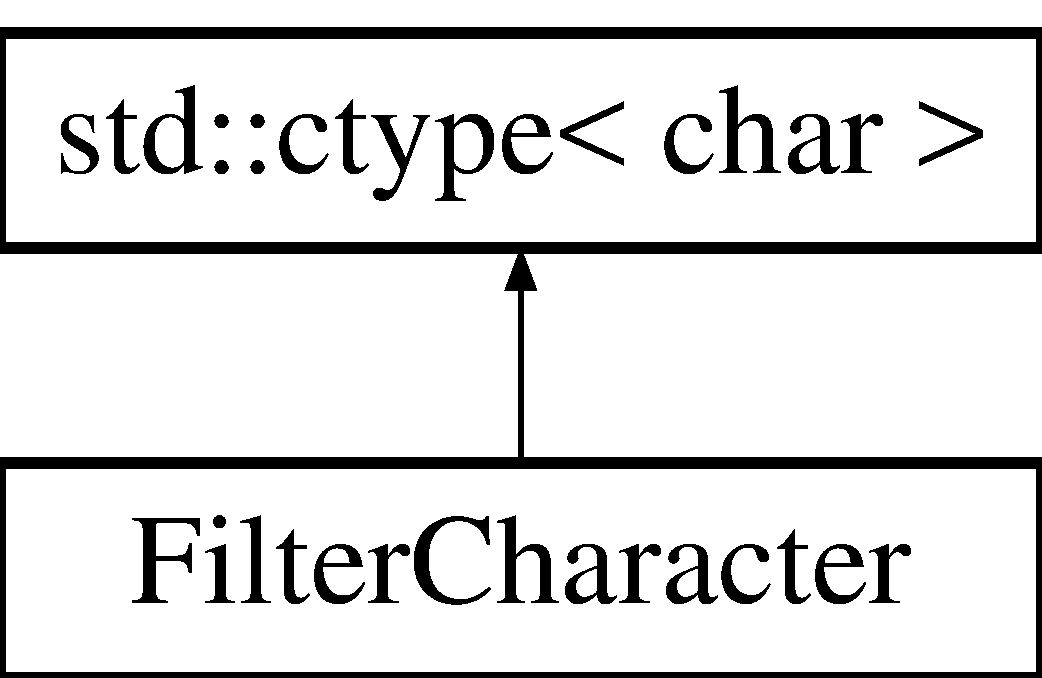
\includegraphics[height=2.000000cm]{db/df5/classFilterCharacter}
\end{center}
\end{figure}
\subsection*{Public Member Functions}
\begin{DoxyCompactItemize}
\item 
\mbox{\Hypertarget{classFilterCharacter_af68a4d80a5ce027e32bcb1174ed7c822}\label{classFilterCharacter_af68a4d80a5ce027e32bcb1174ed7c822}} 
{\bfseries Filter\+Character} (const std\+::string \&chars, int initref=1)
\end{DoxyCompactItemize}


\subsection{Detailed Description}


Definition at line 21 of file U\+Model.\+cpp.



The documentation for this class was generated from the following file\+:\begin{DoxyCompactItemize}
\item 
U\+Model.\+cpp\end{DoxyCompactItemize}

\hypertarget{classUException}{}\section{U\+Exception Class Reference}
\label{classUException}\index{U\+Exception@{U\+Exception}}


\hyperlink{classUException}{U\+Exception} class exception may be throwed by \hyperlink{classUModel}{U\+Model} class method.  




{\ttfamily \#include $<$U\+Model.\+h$>$}

Inheritance diagram for U\+Exception\+:\begin{figure}[H]
\begin{center}
\leavevmode
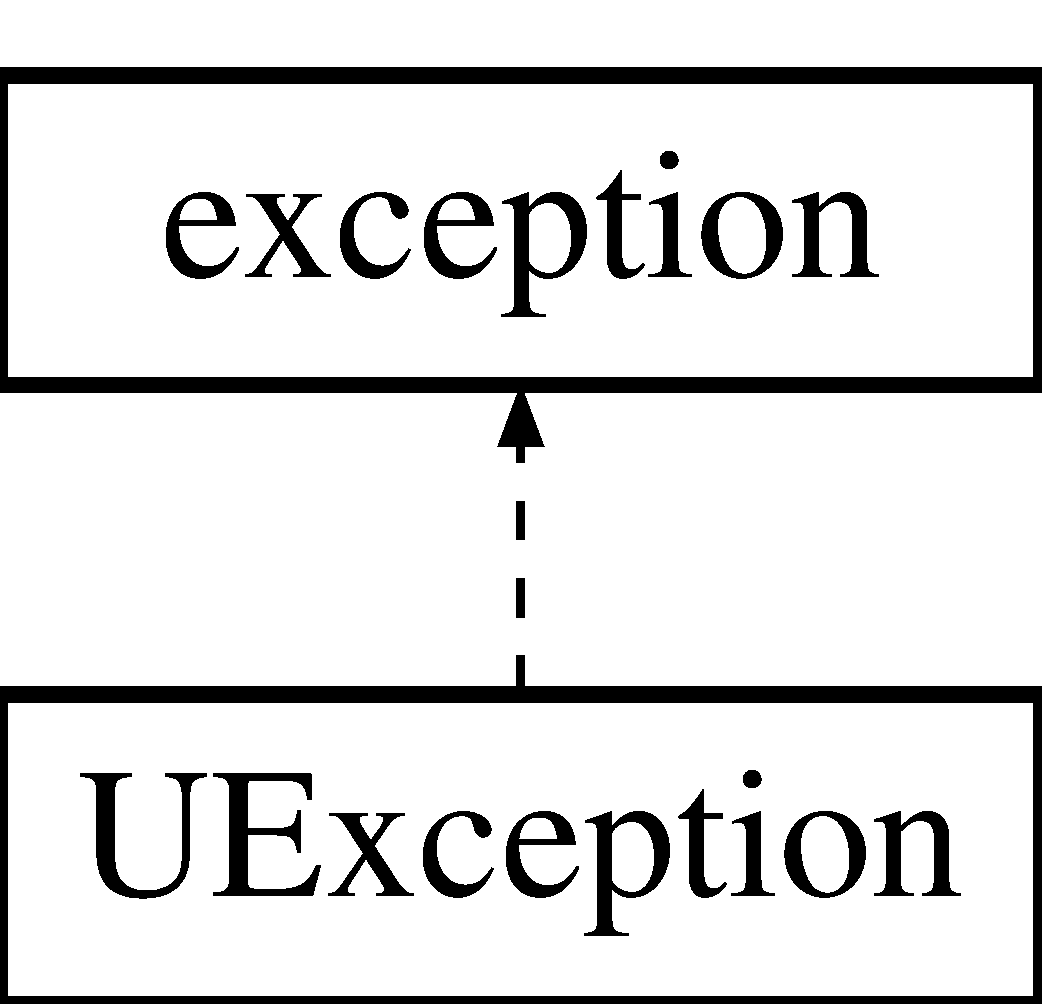
\includegraphics[height=2.000000cm]{dc/d20/classUException}
\end{center}
\end{figure}
\subsection*{Public Member Functions}
\begin{DoxyCompactItemize}
\item 
\mbox{\Hypertarget{classUException_af42bf9ef5955b6c5b72e5752851bc08a}\label{classUException_af42bf9ef5955b6c5b72e5752851bc08a}} 
{\bfseries U\+Exception} (string s)
\item 
\mbox{\Hypertarget{classUException_aee2e2a2e410dcba75cdf97d2b69f77e9}\label{classUException_aee2e2a2e410dcba75cdf97d2b69f77e9}} 
const char $\ast$ {\bfseries what} () const  throw ()
\end{DoxyCompactItemize}
\subsection*{Public Attributes}
\begin{DoxyCompactItemize}
\item 
\mbox{\Hypertarget{classUException_af8f9712643669ed65329aff35cabf6fc}\label{classUException_af8f9712643669ed65329aff35cabf6fc}} 
string {\bfseries s}
\end{DoxyCompactItemize}


\subsection{Detailed Description}
\hyperlink{classUException}{U\+Exception} class exception may be throwed by \hyperlink{classUModel}{U\+Model} class method. 

Definition at line 21 of file U\+Model.\+h.



The documentation for this class was generated from the following files\+:\begin{DoxyCompactItemize}
\item 
U\+Model.\+h\item 
U\+Model.\+cpp\end{DoxyCompactItemize}

\hypertarget{classUModel}{}\section{U\+Model Class Reference}
\label{classUModel}\index{U\+Model@{U\+Model}}


\hyperlink{classUModel}{U\+Model} Class.  




{\ttfamily \#include $<$U\+Model.\+h$>$}

\subsection*{Classes}
\begin{DoxyCompactItemize}
\item 
struct \hyperlink{structUModel_1_1__ODEPAR}{\+\_\+\+O\+D\+E\+P\+AR}
\begin{DoxyCompactList}\small\item\em parameter for O\+DE Solver \end{DoxyCompactList}\item 
struct \hyperlink{structUModel_1_1__REAC}{\+\_\+\+R\+E\+AC}
\item 
struct \hyperlink{structUModel_1_1__SPES}{\+\_\+\+S\+P\+ES}
\item 
struct \hyperlink{structUModel_1_1__TCV}{\+\_\+\+T\+CV}
\end{DoxyCompactItemize}
\subsection*{Public Member Functions}
\begin{DoxyCompactItemize}
\item 
\mbox{\Hypertarget{classUModel_a43f699e133cbab680dc34cbd1f1c90cb}\label{classUModel_a43f699e133cbab680dc34cbd1f1c90cb}} 
bool {\bfseries init\+A\+T\+O\+MS} ()
\item 
bool \hyperlink{classUModel_a29ccc1ecbbd13a3fed4d91395691553b}{init\+S\+P\+E\+CS} (string fspecs)  throw (\+U\+Exception)
\item 
\mbox{\Hypertarget{classUModel_a0f40dac2aa16b1a25ec228c00f961176}\label{classUModel_a0f40dac2aa16b1a25ec228c00f961176}} 
bool \hyperlink{classUModel_a0f40dac2aa16b1a25ec228c00f961176}{init\+R\+A\+T\+ES} (string fratea)  throw (\+U\+Exception)
\begin{DoxyCompactList}\small\item\em read reaction rate file \end{DoxyCompactList}\item 
\mbox{\Hypertarget{classUModel_a83a9a07d304540be3532c4db0c44b648}\label{classUModel_a83a9a07d304540be3532c4db0c44b648}} 
bool \hyperlink{classUModel_a83a9a07d304540be3532c4db0c44b648}{init\+Y\+D\+OT} ()  throw (\+U\+Exception)
\begin{DoxyCompactList}\small\item\em relate each specie(s) to reaction(s). \end{DoxyCompactList}\item 
\mbox{\Hypertarget{classUModel_acca59f52a63d263e3e924ba3b08a0db6}\label{classUModel_acca59f52a63d263e3e924ba3b08a0db6}} 
bool \hyperlink{classUModel_acca59f52a63d263e3e924ba3b08a0db6}{create\+Y\+D\+O\+T\+File} (string s)  throw (\+U\+Exception)
\begin{DoxyCompactList}\small\item\em create file \char`\"{}\+Uode.\+cpp\char`\"{}, which contain defination of Y\+D\+OT(...) \end{DoxyCompactList}\item 
\mbox{\Hypertarget{classUModel_a060609ed8911e53450beda9cefdb6240}\label{classUModel_a060609ed8911e53450beda9cefdb6240}} 
double \hyperlink{classUModel_a060609ed8911e53450beda9cefdb6240}{NH} (double t)
\begin{DoxyCompactList}\small\item\em get Column dnesity of NH at time t \end{DoxyCompactList}\item 
\mbox{\Hypertarget{classUModel_abb8f2d7fad8a36fd3154829b6ea8da5b}\label{classUModel_abb8f2d7fad8a36fd3154829b6ea8da5b}} 
double \hyperlink{classUModel_abb8f2d7fad8a36fd3154829b6ea8da5b}{nH} (double t)
\begin{DoxyCompactList}\small\item\em get number density at time t \end{DoxyCompactList}\item 
\mbox{\Hypertarget{classUModel_a700259282a9a3b6017097ec8612c82cc}\label{classUModel_a700259282a9a3b6017097ec8612c82cc}} 
double \hyperlink{classUModel_a700259282a9a3b6017097ec8612c82cc}{Temp} (double t)
\begin{DoxyCompactList}\small\item\em get temperature at time t \end{DoxyCompactList}\item 
\mbox{\Hypertarget{classUModel_ae2f9952ad7412ee143bf81c65f0db76f}\label{classUModel_ae2f9952ad7412ee143bf81c65f0db76f}} 
double \hyperlink{classUModel_ae2f9952ad7412ee143bf81c65f0db76f}{AV} (double \hyperlink{classUModel_a060609ed8911e53450beda9cefdb6240}{NH})
\begin{DoxyCompactList}\small\item\em F\+U\+N\+C\+T\+I\+ON F\+OR E\+X\+T\+I\+N\+C\+T\+I\+ON AT V-\/\+B\+A\+ND. \end{DoxyCompactList}\item 
\mbox{\Hypertarget{classUModel_a4deca05a74cc3d12049089c1bf028c89}\label{classUModel_a4deca05a74cc3d12049089c1bf028c89}} 
double {\bfseries A\+UV} (double \hyperlink{classUModel_a060609ed8911e53450beda9cefdb6240}{NH})
\item 
\mbox{\Hypertarget{classUModel_a4d49e9a28edb5d0aea7366db053a233d}\label{classUModel_a4d49e9a28edb5d0aea7366db053a233d}} 
void \hyperlink{classUModel_a4d49e9a28edb5d0aea7366db053a233d}{R\+A\+T\+ES} (double t)
\begin{DoxyCompactList}\small\item\em save NH, nH, Temp, AV, Time at time t to \mbox{[}struct \hyperlink{structUModel_1_1__TCV}{\+\_\+\+T\+CV} T\+CV\mbox{]} \end{DoxyCompactList}\item 
\mbox{\Hypertarget{classUModel_a5671676f8fd3c44639c8f373bd5b006b}\label{classUModel_a5671676f8fd3c44639c8f373bd5b006b}} 
double {\bfseries K} (int i, double \hyperlink{classUModel_a700259282a9a3b6017097ec8612c82cc}{Temp}, double \hyperlink{classUModel_ae2f9952ad7412ee143bf81c65f0db76f}{AV})
\item 
\mbox{\Hypertarget{classUModel_a8ba1800cd07a59ae888d1d31d41e03c4}\label{classUModel_a8ba1800cd07a59ae888d1d31d41e03c4}} 
void {\bfseries O\+D\+E\+S\+O\+L\+V\+ER} ()
\item 
\mbox{\Hypertarget{classUModel_a2d3999e57e67fdd956e600d56fc42eb2}\label{classUModel_a2d3999e57e67fdd956e600d56fc42eb2}} 
bool {\bfseries run} ()
\item 
\mbox{\Hypertarget{classUModel_ad5cc4202506cb672dd1a008a8915965a}\label{classUModel_ad5cc4202506cb672dd1a008a8915965a}} 
bool {\bfseries test} ()
\end{DoxyCompactItemize}
\subsection*{Public Attributes}
\begin{DoxyCompactItemize}
\item 
\mbox{\Hypertarget{classUModel_af29c7839f0a1d115eb7a8570bf44da4c}\label{classUModel_af29c7839f0a1d115eb7a8570bf44da4c}} 
map$<$ string, double $>$ {\bfseries A\+T\+O\+MS}
\item 
\mbox{\Hypertarget{classUModel_a634653365e3d4ce42e637291aa940b30}\label{classUModel_a634653365e3d4ce42e637291aa940b30}} 
double {\bfseries init\+Time}
\item 
\mbox{\Hypertarget{classUModel_ac07083e5e31a16452b7d76f1086ad4e1}\label{classUModel_ac07083e5e31a16452b7d76f1086ad4e1}} 
int {\bfseries N\+S\+P\+E\+CS} =0
\item 
\mbox{\Hypertarget{classUModel_ab896ea61c59b3b4175803d168a4fd298}\label{classUModel_ab896ea61c59b3b4175803d168a4fd298}} 
int {\bfseries N\+C\+O\+NS} =0
\item 
\mbox{\Hypertarget{classUModel_a687563585d29e83b3ada8a0c51e8f33c}\label{classUModel_a687563585d29e83b3ada8a0c51e8f33c}} 
int {\bfseries N\+P\+AR} =0
\item 
\mbox{\Hypertarget{classUModel_abdd816110011f5bc8f80ea16864a61c1}\label{classUModel_abdd816110011f5bc8f80ea16864a61c1}} 
double {\bfseries T\+O\+T\+AL} \mbox{[}10\mbox{]}
\item 
\mbox{\Hypertarget{classUModel_af37c95b04367ee27da655a3e9a186745}\label{classUModel_af37c95b04367ee27da655a3e9a186745}} 
double {\bfseries X} \mbox{[}10\mbox{]}
\item 
\mbox{\Hypertarget{classUModel_a1ddeacc4a750d349b34797dd54e9728c}\label{classUModel_a1ddeacc4a750d349b34797dd54e9728c}} 
\hyperlink{structUModel_1_1__SPES}{\+\_\+\+S\+P\+ES} $\ast$ {\bfseries S\+P\+ES}
\item 
\mbox{\Hypertarget{classUModel_a161074ae250acbae3a8b2bd55c94a949}\label{classUModel_a161074ae250acbae3a8b2bd55c94a949}} 
int {\bfseries N\+R\+E\+AC} =0
\item 
\mbox{\Hypertarget{classUModel_afc6da453556a01a5685cb7c2b7318cf9}\label{classUModel_afc6da453556a01a5685cb7c2b7318cf9}} 
\hyperlink{structUModel_1_1__REAC}{\+\_\+\+R\+E\+AC} $\ast$ {\bfseries R\+E\+AC}
\item 
\mbox{\Hypertarget{classUModel_a78f91781f5c783ecdfeedfd3106c7c3a}\label{classUModel_a78f91781f5c783ecdfeedfd3106c7c3a}} 
\hyperlink{structUModel_1_1__TCV}{\+\_\+\+T\+CV} {\bfseries T\+CV}
\item 
double \hyperlink{classUModel_aa8280e76ef6df680f23902d267450c04}{Z\+E\+TA} =1.\+0
\item 
\mbox{\Hypertarget{classUModel_acaed1acb0533429fc4784fb79f0de04c}\label{classUModel_acaed1acb0533429fc4784fb79f0de04c}} 
double \hyperlink{classUModel_acaed1acb0533429fc4784fb79f0de04c}{A\+L\+B\+E\+DO} =0.\+5
\begin{DoxyCompactList}\small\item\em G\+R\+A\+IN A\+L\+B\+E\+DO (F\+OR C\+O\+S\+M\+I\+C-\/\+R\+A\+Y-\/\+I\+N\+D\+U\+C\+ED P\+H\+O\+T\+ON R\+A\+T\+ES) \end{DoxyCompactList}\item 
\mbox{\Hypertarget{classUModel_a52a0fd62c367b920dc639fc56e022133}\label{classUModel_a52a0fd62c367b920dc639fc56e022133}} 
double {\bfseries Y} \mbox{[}1000\mbox{]} =\{0.\+0\}
\item 
\mbox{\Hypertarget{classUModel_a3b789d852868644369e5839199da7646}\label{classUModel_a3b789d852868644369e5839199da7646}} 
double {\bfseries times} \mbox{[}1000\mbox{]}
\item 
\mbox{\Hypertarget{classUModel_ad75bb930f60c12c93600ce93db09efd3}\label{classUModel_ad75bb930f60c12c93600ce93db09efd3}} 
double($\ast$ {\bfseries abuns} )\mbox{[}1000\mbox{]} =N\+U\+LL
\item 
\mbox{\Hypertarget{classUModel_a861ac76efe016adcbb6528a5e15c0808}\label{classUModel_a861ac76efe016adcbb6528a5e15c0808}} 
double {\bfseries H\+N\+Rs} \mbox{[}1000\mbox{]}
\item 
\mbox{\Hypertarget{classUModel_ac7082bd1b75f39d1b349415dc9153e58}\label{classUModel_ac7082bd1b75f39d1b349415dc9153e58}} 
\hyperlink{structUModel_1_1__ODEPAR}{\+\_\+\+O\+D\+E\+P\+AR} {\bfseries O\+D\+E\+P\+AR}
\end{DoxyCompactItemize}


\subsection{Detailed Description}
\hyperlink{classUModel}{U\+Model} Class. 

\hyperlink{classUModel}{U\+Model} object can


\begin{DoxyItemize}
\item parse file
\begin{DoxyItemize}
\item .specs\+: load species to be take into acount to \hyperlink{structUModel_1_1__SPES}{U\+Model\+::\+\_\+\+S\+P\+ES} S\+P\+ES
\item .rates\+: load species to be take into acount to \hyperlink{structUModel_1_1__REAC}{U\+Model\+::\+\_\+\+R\+E\+AC} R\+E\+AC
\end{DoxyItemize}
\item create \hyperlink{Uode_8cpp_source}{Uode.\+cpp} file, define void Y\+D\+OT(...), used as a callback function of O\+DE Solver
\item set time-\/dependent variables at \hyperlink{structUModel_1_1__TCV}{U\+Model\+::\+\_\+\+T\+CV} T\+CV
\begin{DoxyItemize}
\item NH\+: Column dnesity
\begin{DoxyItemize}
\item created by ...
\end{DoxyItemize}
\item nH\+: Number density
\item Temp\+: Temperature
\item AV\+: Extinction at V band
\item K\+: Reaction rates
\item t\+: time
\end{DoxyItemize}
\item run single point chemical evolution model. 
\end{DoxyItemize}

Definition at line 47 of file U\+Model.\+h.



\subsection{Member Function Documentation}
\mbox{\Hypertarget{classUModel_a29ccc1ecbbd13a3fed4d91395691553b}\label{classUModel_a29ccc1ecbbd13a3fed4d91395691553b}} 
\index{U\+Model@{U\+Model}!init\+S\+P\+E\+CS@{init\+S\+P\+E\+CS}}
\index{init\+S\+P\+E\+CS@{init\+S\+P\+E\+CS}!U\+Model@{U\+Model}}
\subsubsection{\texorpdfstring{init\+S\+P\+E\+C\+S()}{initSPECS()}}
{\footnotesize\ttfamily bool U\+Model\+::init\+S\+P\+E\+CS (\begin{DoxyParamCaption}\item[{string}]{fspecs }\end{DoxyParamCaption}) throw  \hyperlink{classUException}{U\+Exception}) }


\begin{DoxyParams}[1]{Parameters}
 & {\em index} & \\
\hline
\mbox{\tt in}  & {\em fspecs} & the species file \\
\hline
\end{DoxyParams}
\begin{DoxyReturn}{Returns}
-\/{\itshape false} fail -\/{\itshape true} succeed 
\end{DoxyReturn}
\begin{DoxyParagraph}{example\+:}

\begin{DoxyCode}
\hyperlink{classUModel_a29ccc1ecbbd13a3fed4d91395691553b}{initSPECS}(\textcolor{stringliteral}{"gasrun.specs"});
\end{DoxyCode}
 
\end{DoxyParagraph}
\begin{DoxyPrecond}{Precondition}
fspecs exist under search path, default \char`\"{}./\char`\"{}read species to be take into acount, and set initial abuandance. 
\end{DoxyPrecond}


Definition at line 85 of file U\+Model.\+cpp.



\subsection{Member Data Documentation}
\mbox{\Hypertarget{classUModel_aa8280e76ef6df680f23902d267450c04}\label{classUModel_aa8280e76ef6df680f23902d267450c04}} 
\index{U\+Model@{U\+Model}!Z\+E\+TA@{Z\+E\+TA}}
\index{Z\+E\+TA@{Z\+E\+TA}!U\+Model@{U\+Model}}
\subsubsection{\texorpdfstring{Z\+E\+TA}{ZETA}}
{\footnotesize\ttfamily double U\+Model\+::\+Z\+E\+TA =1.\+0}

C\+O\+S\+M\+I\+C-\/\+R\+AY I\+O\+N\+I\+S\+A\+T\+I\+ON R\+A\+TE S\+C\+A\+L\+I\+NG F\+A\+C\+T\+OR 

Definition at line 95 of file U\+Model.\+h.



The documentation for this class was generated from the following files\+:\begin{DoxyCompactItemize}
\item 
U\+Model.\+h\item 
U\+Model.\+cpp\end{DoxyCompactItemize}

%--- End generated contents ---

% Index
\backmatter
\newpage
\phantomsection
\clearemptydoublepage
\addcontentsline{toc}{chapter}{Index}
\printindex

\end{document}
